\documentclass{article}

\usepackage{amsmath,amssymb,graphicx,geometry,enumitem,subcaption}
\usepackage{xepersian}

\newcounter{qnumber}
\setcounter{qnumber}{1}

\newcommand{\Q}{
\textbf{سوال \theqnumber)}
\stepcounter{qnumber}
}

\newcommand{\qn}[1]{
\[
\begin{split}
#1
\end{split}
\]
}

\setlength{\parindent}{0mm}
\setlength{\parskip}{3mm}
\settextfont{XB Niloofar}

\begin{document}

\begin{center}
\Large

به نام او

پاسخ تمرینات سری 9
\end{center}

\hrulefill

\large

\Q

\begin{enumerate}[label=\alph*)]
\item
تبدیل فوریه‌ی
$
x(t)+x(t-1)
$
عبارتست از
$$
X(j\omega)[1+\exp(-j\omega)]
$$
که دارای نرخ نایکوئیستی برابر با نرخ نایکوئیست 
$
X(j\omega)
$
است؛ زیرا هرجا که $X(j\omega)$ صفر باشد، 
$
X(j\omega)[1+\exp(-j\omega)]
$
صفر خواهد بود.
\item
تبدیل فوریه‌ی
$
x^2(t)
$
برابر
$
\frac{1}{2\pi}X(j\omega)*X(j\omega)
$
است. بنابراین نرخ نایکوئیست 
$
\frac{1}{2\pi}X(j\omega)*X(j\omega)
$
دو برابر نرخ نایکوئیست
$
X(j\omega)
$
است (به مثال 
$
\Lambda(u)=\Pi(u)*\Pi(u)
$
توجه کنید که 
$
\Pi(u)
$
دارای نرخ 1 و 
$
\Lambda(u)
$
دارای نرخ 2 است). دقت کنید که هر دو سیگنال همچنان باندپایه هستند.
\item
طیف سیگنال 
$
x^2(t)\cos\omega_0 t
$
از روی طیف سیگنال 
$
x^2(t)
$
به راحتی به دست می آید. کافی است طیف 
$
x^2(t)
$
را یکبار به اندازه‌ی $\omega_0$ به چپ و یکبار به راست شیفت دهیم. در این صورت، طیف سیگنال 
$
x^2(t)\cos\omega_0 t
$
از 
$
-2\omega_0
$
تا 
$
2\omega_0
$
کشیده می شود و به نرخ نایکوئیست 
$
4\omega_0
$
منجر خواهد شد.
\end{enumerate}

\Q
\begin{enumerate}[label=\alph*)]
\item
تبدیل فوریه‌ی 
$
\frac{\sin^2 \pi t}{\pi^2t^2}
$
برابر است با
$
\Lambda (\frac{\omega}{2\pi})
$
که
$$
\Lambda (u)=\begin{cases}
1-|u|&,\quad |u|<1\\
0&,\quad \text{سایر جاها}
\end{cases}
$$
\item
برای محاسبه‌ی طیف سیگنال
$
\hat x[n]=x(\frac{n}{F_s})
$
، باید طیف $x(t)$ را روی محور فرکانس، به طور متوالی به اندازه‌ی
$
2k\pi F_s
$
شیفت داده و با هم جمع کنیم. در این صورت به شکل 1 خواهیم رسید.
\begin{figure}[h]
\centering
\begin{subfigure}{0.49\textwidth}
\centering
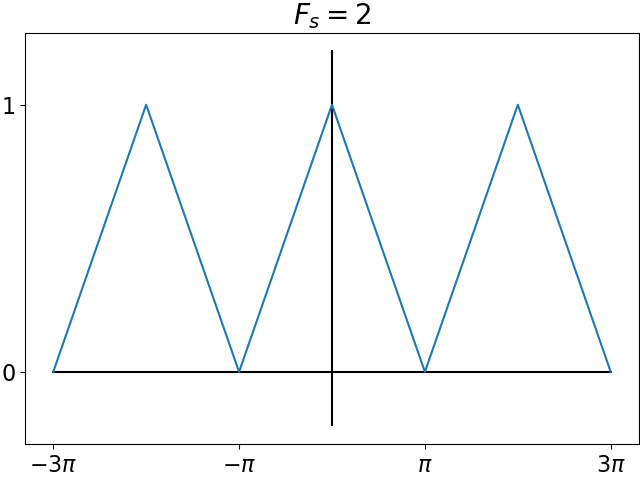
\includegraphics[width=60mm]{fs2.png}
\end{subfigure}
\begin{subfigure}{0.49\textwidth}
\centering
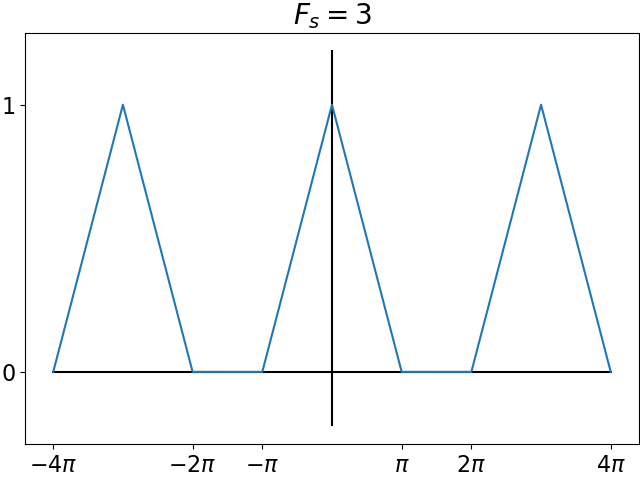
\includegraphics[width=60mm]{fs3.png}
\end{subfigure}
\caption{}
\end{figure}


\end{enumerate}

\Q

\begin{enumerate}[label=\alph*)]
\item
طیف سیگنال نمونه برداری شده 
$
\hat x[n]=x(\frac{n}{F_s})
$
به ازای
$
F_s=1.5
$
در شکل 2 دیده می شود.


\begin{figure}[h]
\centering
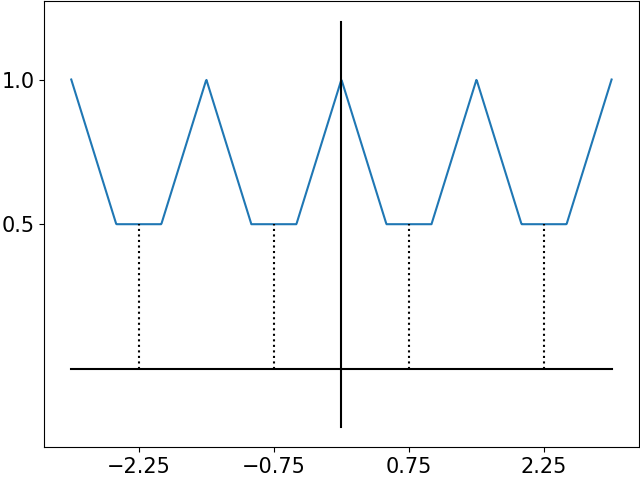
\includegraphics[width=80mm]{aliased.png}
\caption{}
\end{figure}

\item
شکل طیف سیگنال پیوسته 
$
y(t)
$
باید مطابق شکل 3 باشد.
\begin{figure}[h]
\centering
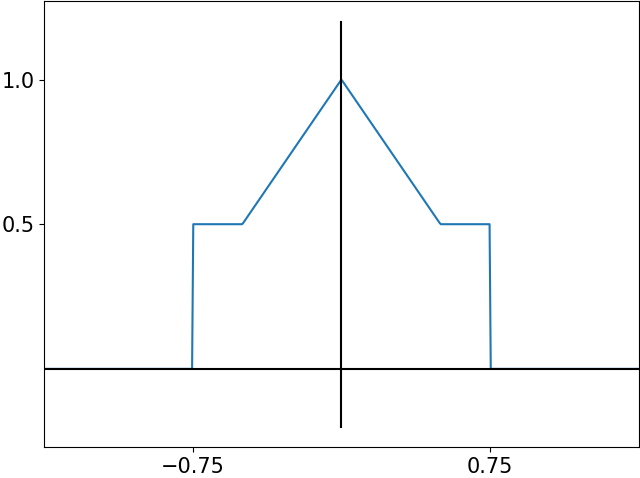
\includegraphics[width=80mm]{y(t).png}
\caption{}
\end{figure}

که رابطه ریاضی آن عبارتست از
$$
Y(j\omega)=\frac{1}{2}\Lambda(\frac{\omega}{\pi})+\frac{1}{2}\Pi(\frac{\omega}{3\pi})
$$
بنابراین
$$
y(t)=\frac{2\sin^2 \frac{\pi t}{2}}{\pi^2t^2}+\frac{\sin \frac{3}{2}\pi t}{2\pi t}
\ne x(t)
$$


\end{enumerate}

\newpage

\newpage

\Q

\begin{enumerate}[label=\alph*)]
\item
سیگنالهای 
$
\sin\frac{4\pi}{3}n
$
و
$
\cos\frac{8\pi}{3}n
$
با دوره‌ی 3 متناوب هستند؛ پس 
$
x[n]
$
نیز با دوره ی 3 متناوب است. بنابراین
$$
\omega_0=\frac{2\pi}{3}
$$

\qn{
x[n]&=\sin\frac{4\pi}{3}n+\cos\frac{8\pi}{3}n
\\&=
\frac{1}{2j}e^{j\frac{4\pi}{3}n}
-
\frac{1}{2j}e^{-j\frac{4\pi}{3}n}
+
\frac{1}{2}e^{j\frac{8\pi}{3}n}
+
\frac{1}{2}e^{-j\frac{8\pi}{3}n}
\\&=
\frac{1}{2j}e^{j\frac{4\pi}{3}n}
-
\frac{1}{2j}e^{-j\frac{4\pi}{3}n}
+
\frac{1}{2}e^{j\frac{2\pi}{3}n}
+
\frac{1}{2}e^{-j\frac{2\pi}{3}n}
\\&=
\frac{1}{2j}e^{-j\frac{2\pi}{3}n}
-
\frac{1}{2j}e^{j\frac{2\pi}{3}n}
+
\frac{1}{2}e^{j\frac{2\pi}{3}n}
+
\frac{1}{2}e^{-j\frac{2\pi}{3}n}
}
و خواهیم داشت
\qn{
a_0=0\quad,\quad a_1=\frac{1}{2}-\frac{1}{2j}\quad,\quad a_2=a_{-1}=\frac{1}{2}+\frac{1}{2j}
}

\item
این سیگنال متناوب نیست؛ زیرا دوره تناوب اساسی آن باید مضرب صحیحی از عدد غیرگویای 
$
\frac{2\pi}{3}
$
باشد.
\item
بنا به تعریف
\qn{
a_k&=\frac{1}{N}\sum_{n=0}^{N-1}x[n]e^{-jk\omega_0n}
\\&=\frac{1}{4}\sum_{n=0}^3x[n]e^{-jkn\frac{\pi}{2}}
\\&=\frac{1}{4}\left[
1-e^{-jk\frac{\pi}{2}}+2e^{-jk2\frac{\pi}{2}}+3e^{-jk3\frac{\pi}{2}}
\right]
\\&=\frac{1}{4}\left[
1-e^{-jk\frac{\pi}{2}}+2(-1)^k+3e^{jk\frac{\pi}{2}}
\right]
}

\item
این سیگنال دارای دوره تناوب اساسی 3 است؛ زیرا
\qn{
x[n+3]&=
\sin \frac{2\pi}{3}(n+3)^2
=
\sin \frac{2\pi}{3}(n^2+6n+9)
\\&=
\sin (\frac{2\pi}{3}n^2+4\pi n+6\pi)
=
\sin \frac{2\pi}{3}n^2=x[n]
}
بنابراین
\qn{
a_k&=\frac{1}{N}\sum_{n=0}^{N-1}x[n]e^{-jk\omega_0n}
\\&=\frac{1}{3}\sum_{n=0}^2x[n]e^{-jkn\frac{2\pi}{3}}
\\&=\frac{1}{3}\left[
\frac{\sqrt 3}{2}e^{-jk\frac{2\pi}{3}}+\frac{\sqrt 3}{2}e^{-jk\frac{4\pi}{3}}
\right]
\\&=\frac{1}{3}\left[
\frac{\sqrt 3}{2}e^{-jk\frac{2\pi}{3}}+\frac{\sqrt 3}{2}e^{jk\frac{2\pi}{3}}
\right]
\\&=\frac{\cos \frac{2k\pi}{3}}{\sqrt 3}
}
\end{enumerate}

\Q

اگر ضرایب سری فوریه سیگنال 
$
(-1)^nx[n]
$
را
$
b_k
$
بنامیم، در این صورت،

الف) بر طبق خواص
$$
b_k=a_{k-{N\over 2}}
$$

ب)$a_k$ با دوره‌ی $N$ متناوب است. اکنون فرض کنید ضرایب $x[n]$ را با دوره‌ی تناوب $2N$ محاسبه کرده و آن را $c_k$ نامیده ایم. در این صورت:
\qn{
&a_k={1\over N}\sum_{n=0}^{{N}-1}x[n]e^{-j{2\pi\over N}kn}
\\&c_k={1\over 2N}\sum_{n=0}^{{2N}-1}x[n]e^{-j{\pi\over N}kn}
\\&=
{1\over 2N}\sum_{n=0}^{N-1}x[n]e^{-j{\pi\over N}kn}
+
{1\over 2N}\sum_{n=N}^{2N-1}x[n]e^{-j{\pi\over N}kn}
\\&=
{1\over 2N}\sum_{n=0}^{N-1}x[n]e^{-j{\pi\over N}kn}
+
{1\over 2N}\sum_{m=0}^{N-1}x[m+N]e^{-j{\pi\over N}k(m+N)}
\\&=
{1\over 2N}\sum_{n=0}^{N-1}x[n]e^{-j{\pi\over N}kn}
+
{1\over 2N}\sum_{n=0}^{N-1}x[n](-1)^ke^{-j{\pi\over N}kn}
\\&=
{1\over 2N}\sum_{n=0}^{N-1}x[n][1+(-1)^k]e^{-j{\pi\over N}kn}
}
بنابراین
$
c_{2k}=a_k
$
و 
$
c_{2k+1}=0
$
.
از طرفی $(-1)^n$، شیفتی به اندازه‌ی نصف دوره تناوب یعنی 
$
{2N\over 2}=N
$
 در حوزه‌ی فوریه تحمیل می کند؛ پس:
$$
b_k=\begin{cases}
0&,\quad \text{k زوج}
\\
a_{k-N\over 2}&,\quad \text{k فرد}
\end{cases}
$$

\Q

بر اساس رابطه‌ی آنالیز سری فوریه
$$
a_k=\frac{1}{N}\sum_{n=0}^{N-1}x[n]e^{-jkn\omega_0}
=\frac{1}{6}\sum_{n=0}^{5}x[n]e^{-jkn\frac{\pi}{3}}
$$

\begin{enumerate}
\item
(!!)
\item
$
a_3=\frac{1}{3}
$
\item
$
a_0=a_5=1
$
\item
\qn{
\sum _{n=0}^5|x[n]|^2&=6\sum _{k=0}^5|a_k|^2
\\&=\frac{38}{3}
}
\end{enumerate}
بنابراین
\qn{
\sum _{k=0}^5|a_k|^2&=a_0^2+a_1^2+a_2^2+a_3^2+a_4^2+a_5^2
\\&=1+a_1^2+a_2^2+\frac{1}{9}+a_4^2+1=
\frac{19}{9}
\\&\implies a_1^2+a_2^2+a_4^2=0
\\&\implies a_1=a_2=a_4=0
}
و نهایتأ
\qn{
x[n]&=\sum_{k=0}^{N-1} a_ke^{jkn\omega_0}
=
\sum_{k=0}^{5} a_ke^{jkn\frac{\pi}{3}}
\\&=
1+\frac{1}{3}e^{j3n\frac{\pi}{3}}+e^{j5n\frac{\pi}{3}}
\\&=
1+\frac{(-1)^n}{3}+e^{j5n\frac{\pi}{3}}
}

\Q

اگر ورودی گسسته‌ و متناوب
$
x[n]
$
با ضرایب سری فوریه‌ی 
$
a_k
$
و فرکانس اساسی $\omega_0$، وارد سیستم LTI با پاسخ فرکانسی
$
H(e^{j\omega})
$
شود، خروجی متناوب و دارای ضرایب سری فوریه‌ی 
$
a_kH(e^{jk\omega_0})
$
خواهد بود. بر این مبنا، پاسخ فرکانسی سیستم برابر است با
$$
H(e^{j\omega})=\frac{1}{1-\frac{1}{3}e^{-j\omega}}.
$$
همچنین، برای ورودی داریم
$
\omega_0=\frac{\pi}{2}
$
و ضرایب سری فوریه‌ی آن عبارتست از
\qn{
a_k&=\frac{1}{N}\sum_{n=0}^{N-1}x[n]e^{-jkn\omega_0}
\\&=\frac{1}{4}\sum_{n=0}^{3}x[n]e^{-jkn\frac{\pi}{2}}
\\&=\frac{1}{4}\left[1+2e^{-jk\frac{\pi}{2}}\right]
}
بنابراین ضرایب سری فوریه‌ی خروجی به صورت زیرند:
$$
b_k=a_kH(e^{jk\omega_0})=
\frac{1+2e^{-jk\frac{\pi}{2}}}{4-\frac{4}{3}e^{-jk\frac{\pi}{2}}}
$$

\end{document}